\documentclass[12pt,a4paper]{article}

\usepackage{fontspec}
\setmainfont{DejaVu Serif}
\setsansfont{DejaVu Sans}
\setmonofont{DejaVu Sans Mono}
\usepackage[a4paper,margin=2.3cm]{geometry}
\usepackage{graphicx}
\usepackage{booktabs}
\usepackage{array}
\usepackage{tabularx}
\usepackage{longtable}
\usepackage{amsmath,amssymb}
\usepackage{xcolor}
\usepackage{float}
\usepackage{enumitem}
\usepackage{caption}
\usepackage{microtype}
\usepackage{fancyhdr}
\usepackage{tocloft}
\usepackage[hidelinks]{hyperref}
\usepackage{xurl}
\usepackage{listings}
\usepackage{tikz}
\usetikzlibrary{arrows.meta,positioning,shapes.geometric}

\graphicspath{{docs/images/}}
\setlength{\parindent}{1.2em}
\setlength{\parskip}{0.35em}
\setlist{nosep}
\captionsetup{font=small,labelfont=bf}
\setlength{\emergencystretch}{2em}
\setlength{\cftbeforesecskip}{0.4em}
\setlength{\cftsecnumwidth}{2.6em}
\setlength{\cftsubsecnumwidth}{3.2em}

\definecolor{hcmusblue}{HTML}{0A4B8F}
\definecolor{codegray}{HTML}{F3F5F6}
\definecolor{rulegray}{HTML}{D4DADD}
\newcolumntype{Y}{>{\raggedright\arraybackslash}X}
\newcolumntype{P}[1]{>{\raggedright\arraybackslash}p{#1}}

\pagestyle{fancy}
\fancyhf{}
\lhead{AI101 Lab 1 -- Searching}
\rhead{Group 1}
\cfoot{\thepage}
\setlength{\headheight}{15pt}
\renewcommand{\headrulewidth}{0.4pt}

\hypersetup{
    pdftitle={Lab 1 - Searching: Saigon Route Lab},
    pdfauthor={Group 1},
    pdfsubject={Tourist route planning with graph-search algorithms}
}

\lstset{
    basicstyle=\ttfamily\small,
    backgroundcolor=\color{codegray},
    frame=single,
    rulecolor=\color{rulegray},
    breaklines=true,
    columns=fullflexible,
    showstringspaces=false,
    aboveskip=0.8em,
    belowskip=0.8em
}

\tikzset{
    process/.style={rectangle, rounded corners=2pt, draw=hcmusblue,
        minimum height=0.85cm, text width=4.2cm, align=center,
        font=\small, fill=blue!3},
    decision/.style={diamond, draw=hcmusblue, aspect=2.2,
        text width=2.4cm, align=center, font=\small, fill=blue!3},
    flow/.style={-{Latex[length=2.2mm]}, semithick, draw=hcmusblue}
}

\begin{document}

\hypersetup{pageanchor=false}
\begin{titlepage}
    \centering
    
\includegraphics[width=11cm]{university_logo_wordmark.png}\par
    \vspace{0.4cm}
    {\Large\textbf{VNUHCM -- UNIVERSITY OF SCIENCE}\par}
    \vspace{0.25cm}
    {\large Faculty of Information Technology\par}
    \vspace{0.15cm}
    {\large Course: Introduction to Artificial Intelligence\par}

    \vfill

    {\Huge\bfseries LAB 1 -- SEARCHING\par}
    \vspace{0.35cm}
    {\LARGE\bfseries SAIGON ROUTE LAB\par}
    \vspace{0.55cm}
    {\large Tourist Route Planner for Visiting Multiple Landmarks\\
    in Ho Chi Minh City\par}

    \vfill

    {\large\bfseries Group ID: 1\par}
    \vspace{0.3cm}
    \renewcommand{\arraystretch}{1.28}
    \begin{tabular}{>{\bfseries}l l}
        24127052 & Phùng Bảo Khang \\
        24127069 & Thái Kiệt \\
        24127167 & Nguyễn Đăng Hậu \\
        24127257 & Nguyễn Thành Trung \\
        24127378 & Nguyễn Huy Hoàng \\
    \end{tabular}

    \vfill
    {\large Ho Chi Minh City, August 2026\par}
\end{titlepage}
\hypersetup{pageanchor=true}

\pagenumbering{roman}
{\small\tableofcontents}
\clearpage
\pagenumbering{arabic}

\section{Group Introduction and Completion}

\subsection{Member responsibilities}

Table~\ref{tab:members} records the principal responsibility assigned to each
member. Every listed work package is implemented and integrated in the final
application; completion denotes the assigned work, not a percentage of total
individual authorship.

\begin{table}[H]
    \centering
    \caption{Group members, responsibilities, and completion.}
    \label{tab:members}
    \renewcommand{\arraystretch}{1.15}
    \small
    \begin{tabularx}{\textwidth}{P{2.1cm} P{3.3cm} Y c}
        \toprule
        \textbf{Student ID} & \textbf{Full name} &
        \textbf{Main contribution} & \textbf{Done} \\
        \midrule
        24127378 & Nguyễn Huy Hoàng &
        BFS, Vietnamese traffic context, report introduction & 100\% \\
        24127167 & Nguyễn Đăng Hậu &
        DFS, graph model, dataset, and cost function & 100\% \\
        24127257 & Nguyễn Thành Trung &
        UCS, route explanation, and algorithm analysis & 100\% \\
        24127052 & Phùng Bảo Khang &
        $A^*$, heuristic, GUI, and visualization & 100\% \\
        24127069 & Thái Kiệt &
        Dijkstra, Greedy Best-First, and multi-location optimization & 100\% \\
        \bottomrule
    \end{tabularx}
\end{table}

\subsection{Requirement completion}

\begin{table}[H]
    \centering
    \caption{Implementation evidence for the Lab 1 requirements.}
    \label{tab:completion}
    \renewcommand{\arraystretch}{1.15}
    \small
    \begin{tabularx}{\textwidth}{P{4.2cm} Y P{2cm}}
        \toprule
        \textbf{Requirement} & \textbf{Evidence} & \textbf{Status} \\
        \midrule
        Vietnamese traffic scenario & 24 HCMC landmarks and OSM-derived roads & Complete \\
        Graph, dataset, and cost & 481 nodes, 995 directed edges, weighted traffic cost & Complete \\
        BFS, DFS, UCS, and $A^*$ & Independent implementations with shared contracts & Complete \\
        Two additional algorithms & Dijkstra and Greedy Best-First & Complete \\
        Multi-location planning & Nearest Neighbor and Exact Brute Force & Complete \\
        GUI and visualization & React, Leaflet, REST, and WebSocket step stream & Complete \\
        Explanation and alternatives & Named roads, congestion, guarantee, and baseline comparison & Complete \\
        Verification & 70 tests, all-pair audit, and frontend production build & Complete \\
        \bottomrule
    \end{tabularx}
\end{table}

\section{Problem Context}

Tourists often want to visit several attractions in central Ho Chi Minh City
in one trip. The physically shortest route may be unsuitable because major
roads can be slow during rush hour, rain can increase travel time and road
risk, and one-way streets constrain movement. The project therefore recommends
routes using distance, estimated travel time, congestion, and risk instead of
distance alone.

The application supports two related tasks:

\begin{enumerate}
    \item find a route from one selected landmark to another;
    \item choose an efficient visiting order and complete route for several
          required landmarks.
\end{enumerate}

This is a Vietnamese traffic problem rather than an abstract maze. Landmark
names, road geometry, road classes, and directionality are grounded in Ho Chi
Minh City data.

\section{Problem Modeling}

The traffic network is a directed weighted graph $G=(V,E)$.

\begin{itemize}
    \item \textbf{State:} the current routable road node.
    \item \textbf{Initial state:} the unique road node assigned to the selected
          starting landmark.
    \item \textbf{Goal test:} the current node equals the destination node.
    \item \textbf{Action:} follow one outgoing directed road edge.
    \item \textbf{Path:} an ordered node sequence connected by valid edges.
    \item \textbf{Path cost:} the sum of weighted edge costs.
\end{itemize}

Each edge stores physical distance, estimated travel time, congestion, risk,
road type, road name, one-way metadata, and drawing geometry. Algorithms never
infer a reverse edge: reverse travel is possible only when the loader provides
that directed edge.

\begin{table}[H]
    \centering
    \caption{Runtime edge fields.}
    \label{tab:edge-fields}
    \renewcommand{\arraystretch}{1.15}
    \small
    \begin{tabularx}{\textwidth}{P{3.2cm} P{3.2cm} Y}
        \toprule
        \textbf{Field} & \textbf{Unit or range} & \textbf{Meaning} \\
        \midrule
        \texttt{distance\_km} & km, non-negative & Physical road length \\
        \texttt{time\_min} & minutes, non-negative & Estimated travel time \\
        \texttt{congestion} & 1 to 5 & Scenario traffic level \\
        \texttt{risk} & 0 to 5 & Road-class and weather penalty \\
        \texttt{road\_type} & text & OpenStreetMap highway class \\
        \texttt{oneway} & Boolean metadata & Whether reverse travel is prohibited \\
        \texttt{geometry} & coordinate list & Line drawn by Leaflet \\
        \bottomrule
    \end{tabularx}
\end{table}

\section{Dataset}

The source GeoJSON was produced from OpenStreetMap using the group's OSMnx
tooling. The extracts contain 1,075 directed road features, 519 intersection
records, and approximately 95.083 km of road geometry. The loader normalizes
duplicate endpoint pairs, joins two adjacent major components, and retains the
largest strongly connected graph.

\begin{table}[H]
    \centering
    \caption{Final graph dimensions.}
    \label{tab:graph-size}
    \renewcommand{\arraystretch}{1.15}
    \begin{tabular}{lr}
        \toprule
        \textbf{Property} & \textbf{Value} \\
        \midrule
        Routable nodes & 481 \\
        Directed edges & 995 \\
        One-way directed edges & 403 \\
        Tourist landmarks & 24 \\
        Unique assigned landmark nodes & 24 \\
        Traffic profiles & 3 \\
        \bottomrule
    \end{tabular}
\end{table}

Every landmark is assigned to a unique nearby routable node so that two
required stops cannot collapse into one visit. Marker-to-node offsets are shown
as dashed access lines in the GUI. The mean offset is about 100 m and the
maximum is 383.5 m for Ben Thanh Market. These access offsets are not included
in road-route totals and remain a documented limitation.

The two source boundaries are separately clipped. One bidirectional boundary
connection, represented by two directed simulated edges, joins their major road
components. The GUI identifies this assumption as \emph{Boundary connector}.

The 24 landmarks include Ben Thanh Market, Independence Palace, War Remnants
Museum, Notre Dame Cathedral, Central Post Office, Nguyen Hue Walking Street,
Bach Dang Wharf, Saigon Opera House, Tao Dan Park, Fine Arts Museum, Tan Dinh
Church, Saigon Zoo, Vinh Nghiem Pagoda, and other central destinations. The
complete machine-readable list is stored in \texttt{data/landmarks.json}.

\section{Cost Function and Traffic Conditions}

For an edge $e$, the configurable weighted cost is

\begin{equation}
    C(e)=\alpha d(e)+\beta t(e)+\gamma q(e)+\delta r(e),
    \label{eq:cost}
\end{equation}

where $d$ is distance in kilometres, $t$ is estimated time in minutes, $q$ is
congestion, and $r$ is risk. Every term and weight is non-negative; therefore,
UCS and Dijkstra satisfy their non-negative-cost optimality condition.

\begin{table}[H]
    \centering
    \caption{Cost-criterion presets.}
    \label{tab:presets}
    \renewcommand{\arraystretch}{1.12}
    \small
    \begin{tabularx}{\textwidth}{lrrrrY}
        \toprule
        \textbf{Preset} & $\alpha$ & $\beta$ & $\gamma$ & $\delta$ & \textbf{Purpose} \\
        \midrule
        Balanced & 1.00 & 0.40 & 0.08 & 0.12 & Trade off all four factors \\
        Fastest & 0.20 & 1.20 & 0.04 & 0.08 & Emphasize estimated time \\
        Shortest & 1.50 & 0.05 & 0.01 & 0.03 & Emphasize distance \\
        Low congestion & 0.70 & 0.30 & 0.25 & 0.15 & Avoid congested roads \\
        Low risk & 0.50 & 0.30 & 0.08 & 0.80 & Avoid higher-risk roads \\
        \bottomrule
    \end{tabularx}
\end{table}

The \textbf{normal} profile uses base road-class values. \textbf{Rush hour}
increases time, congestion, and risk, with a larger time multiplier on primary
and secondary roads. \textbf{Rainy} increases time, congestion, and risk using
a deterministic hybrid scenario. These are reproducible academic scenarios,
not live sensor measurements.

\section{Algorithm Principles}

The group designed the graph in Figure~\ref{fig:example-graph} for unit tests
and step-by-step video explanation. Route $A\rightarrow B\rightarrow G$ has two
edges and cost 9, while $A\rightarrow C\rightarrow D\rightarrow G$ has three
edges and cost 3. The example exposes the difference between structural,
cost-aware, and heuristic search.

\begin{figure}[H]
    \centering
    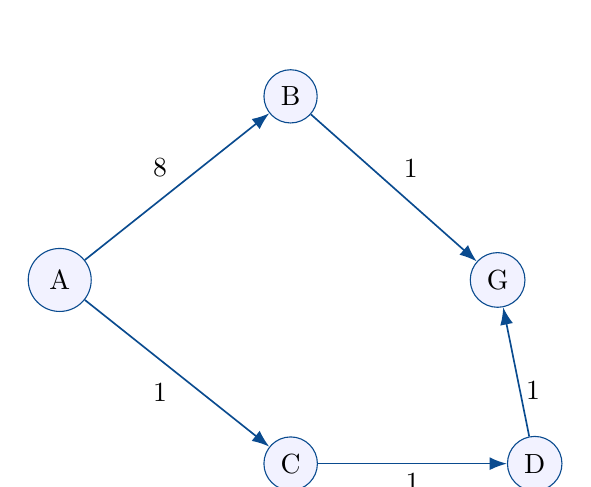
\begin{tikzpicture}[node distance=1.8cm and 2.4cm]
        \node[circle,draw=hcmusblue,fill=blue!5,minimum size=8mm] (A) {A};
        \node[circle,draw=hcmusblue,fill=blue!5,above right=of A] (B) {B};
        \node[circle,draw=hcmusblue,fill=blue!5,below right=of A] (C) {C};
        \node[circle,draw=hcmusblue,fill=blue!5,right=of C] (D) {D};
        \node[circle,draw=hcmusblue,fill=blue!5,right=4.8cm of A] (G) {G};
        \draw[flow] (A) -- node[above left]{8} (B);
        \draw[flow] (B) -- node[above right]{1} (G);
        \draw[flow] (A) -- node[below left]{1} (C);
        \draw[flow] (C) -- node[below]{1} (D);
        \draw[flow] (D) -- node[below right]{1} (G);
    \end{tikzpicture}
    \caption{Group-designed graph with competing minimum-edge and minimum-cost routes.}
    \label{fig:example-graph}
\end{figure}

\begin{table}[H]
    \centering
    \caption{Expansion order and result on the group-designed graph.}
    \label{tab:example-results}
    \renewcommand{\arraystretch}{1.12}
    \scriptsize
    \begin{tabularx}{\textwidth}{P{2cm} Y P{3.7cm} r}
        \toprule
        \textbf{Algorithm} & \textbf{Expansion or pop order} &
        \textbf{Final route} & \textbf{Cost} \\
        \midrule
        BFS & \texttt{A, B, C, G} & \texttt{A -> B -> G} & 9 \\
        DFS & \texttt{A, B, G} & \texttt{A -> B -> G} & 9 \\
        UCS & \texttt{A(0), C(1), D(2), G(3)} by $g$ &
        \texttt{A -> C -> D -> G} & 3 \\
        $A^*$ & \texttt{A(2), C(3), D(3), G(3)} by $f=g+h$ &
        \texttt{A -> C -> D -> G} & 3 \\
        Dijkstra & \texttt{A(0), C(1), D(2), G(3)} by distance label &
        \texttt{A -> C -> D -> G} & 3 \\
        Greedy & \texttt{A(2), B(0), G(0)} by $h$ &
        \texttt{A -> B -> G} & 9 \\
        \bottomrule
    \end{tabularx}
\end{table}

\subsection{Breadth-First Search}

BFS uses a FIFO queue and expands the shallowest discovered node. It is
complete on this finite graph and optimal only by edge count when every action
has equal cost. It does not generally minimize the traffic cost in
Equation~\ref{eq:cost}.

\subsection{Depth-First Search}

DFS uses a LIFO stack and follows one branch before backtracking. A discovered
set prevents cycles. It is complete for this finite explicit graph but does not
guarantee a short, fast, or low-cost route.

\subsection{Uniform Cost Search}

UCS orders the frontier by accumulated cost $g(n)$. It stops only when the goal
is removed from the priority queue with its best cost. With non-negative edge
costs, it is complete and optimal. The project contains a goal-directed UCS
implementation with its own trace.

\subsection{\texorpdfstring{$A^*$}{A-star} Search}

$A^*$ orders nodes by

\begin{equation}
    f(n)=g(n)+h(n), \qquad
    h(n)=\alpha\,\operatorname{HaversineDistance}(n,\text{goal}).
\end{equation}

Haversine distance never exceeds road distance, and every other cost term is
non-negative. The heuristic is therefore admissible. It is also consistent:
the metric triangle inequality and the edge cost lower bound imply
$h(n)\leq C(n,n')+h(n')$. Exhaustive checks over every graph edge, all 24
landmark goals, and all five presets found zero consistency violations.

\subsection{Dijkstra's Algorithm}

Dijkstra also expands the lowest accumulated-cost node. In addition to
point-to-point routing, its module exposes a single-source helper used to cache
pairwise paths for multi-location optimization. It is complete and optimal for
non-negative edge costs.

\subsection{Greedy Best-First Search}

Greedy orders the frontier only by $h(n)$. It may expand far fewer nodes but
ignores accumulated traffic cost when deciding where to explore. A closed set
ensures termination on the finite graph; route optimality is not guaranteed.

\subsection{Theoretical comparison}

\begin{table}[H]
    \centering
    \caption{Theoretical properties used in the application.}
    \label{tab:theory}
    \renewcommand{\arraystretch}{1.12}
    \scriptsize
    \begin{tabularx}{\textwidth}{P{1.8cm} P{3.1cm} P{2.4cm} P{2.7cm} Y}
        \toprule
        \textbf{Algorithm} & \textbf{Worst-case time} & \textbf{Memory} &
        \textbf{Complete here} & \textbf{Cost-optimal} \\
        \midrule
        BFS & $O(V+E)$ & $O(V)$ & Yes & Only by edge count \\
        DFS & $O(V+E)$ & $O(V)$ & Yes, finite graph & No \\
        UCS & $O((V+E)\log V)$ & $O(V)$ & Yes & Yes, non-negative cost \\
        $A^*$ & $O((V+E)\log V)$ graph bound & $O(V)$ & Yes & Yes, admissible heuristic \\
        Dijkstra & $O((V+E)\log V)$ & $O(V)$ & Yes & Yes, non-negative cost \\
        Greedy & $O((V+E)\log V)$ & $O(V)$ & Yes, finite graph & No \\
        \bottomrule
    \end{tabularx}
\end{table}

\section{Multi-Location Optimization}

Pairwise shortest paths between important nodes are computed with cached
single-source Dijkstra runs.

\begin{itemize}
    \item \textbf{Nearest Neighbor} repeatedly visits the currently cheapest
          unvisited waypoint. It is deterministic and efficient but approximate.
    \item \textbf{Exact Brute Force} evaluates every waypoint permutation when
          the count is at most eight. It guarantees the best ordering for the
          reduced pairwise shortest-path problem and has factorial complexity.
\end{itemize}

Both methods support a fixed final landmark and returning to the start.
Duplicate waypoints are removed in input order, and an unreachable mandatory
segment produces an explicit failure result. For $k$ required waypoints,
Nearest Neighbor needs $O(k^2)$ route-choice work after pairwise preprocessing,
whereas Exact Brute Force evaluates $k!$ orders.

\section{Program Flow and Architecture}

Figure~\ref{fig:architecture} summarizes the separation between the React GUI,
FastAPI service, search modules, cost profiles, and OSM graph.

\begin{figure}[H]
    \centering
    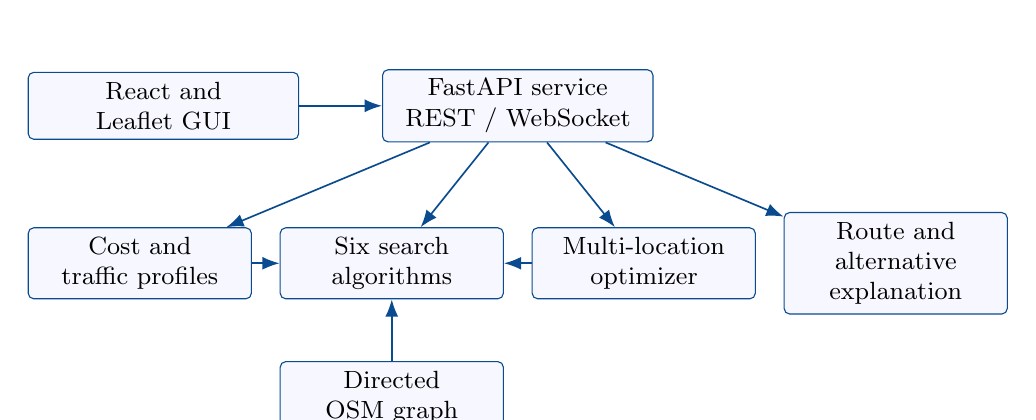
\begin{tikzpicture}[x=1cm,y=1cm]
        \node[process,text width=3.2cm] at (-4.5,0) (gui) {React and Leaflet GUI};
        \node[process,text width=3.2cm] at (0,0) (api) {FastAPI service\\REST / WebSocket};
        \node[process,text width=2.6cm] at (-4.8,-2) (cost) {Cost and traffic profiles};
        \node[process,text width=2.6cm] at (-1.6,-2) (search) {Six search algorithms};
        \node[process,text width=2.6cm] at (1.6,-2) (multi) {Multi-location optimizer};
        \node[process,text width=2.6cm] at (4.8,-2) (explain) {Route and alternative explanation};
        \node[process,text width=2.6cm] at (-1.6,-3.7) (graph) {Directed OSM graph};
        \draw[flow] (gui) -- (api);
        \draw[flow] (api) -- (cost);
        \draw[flow] (api) -- (search);
        \draw[flow] (api) -- (multi);
        \draw[flow] (api) -- (explain);
        \draw[flow] (graph) -- (search);
        \draw[flow] (cost) -- (search);
        \draw[flow] (multi) -- (search);
    \end{tikzpicture}
    \caption{Application architecture and principal data flow.}
    \label{fig:architecture}
\end{figure}

The common point-to-point search flow is shown in
Figure~\ref{fig:search-flow}. Every expansion can be serialized as a shared
trace step containing the current node, frontier, visited set, parent update,
and relevant $g$, $h$, and $f$ values.

\begin{figure}[H]
    \centering
    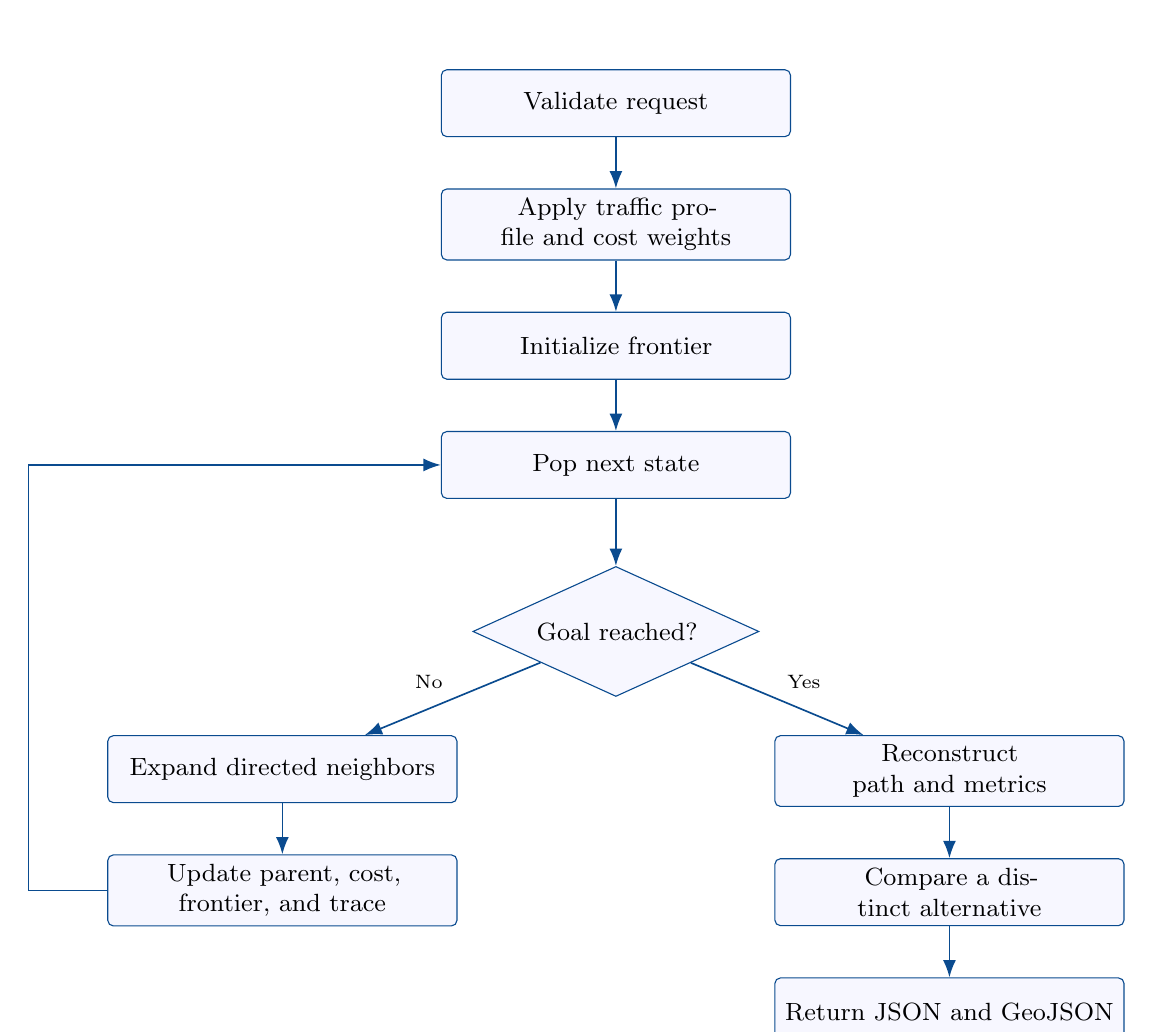
\begin{tikzpicture}[node distance=0.65cm]
        \node[process] (request) {Validate request};
        \node[process,below=of request] (profile) {Apply traffic profile and cost weights};
        \node[process,below=of profile] (init) {Initialize frontier};
        \node[process,below=of init] (pop) {Pop next state};
        \node[decision,below=0.85cm of pop] (goal) {Goal reached?};
        \node[process,below left=0.9cm and 1.1cm of goal] (expand) {Expand directed neighbors};
        \node[process,below=of expand] (update) {Update parent, cost, frontier, and trace};
        \node[process,below right=0.9cm and 1.1cm of goal] (path) {Reconstruct path and metrics};
        \node[process,below=of path] (alternative) {Compare a distinct alternative};
        \node[process,below=of alternative] (return) {Return JSON and GeoJSON};
        \draw[flow] (request) -- (profile);
        \draw[flow] (profile) -- (init);
        \draw[flow] (init) -- (pop);
        \draw[flow] (pop) -- (goal);
        \draw[flow] (goal) -- node[above left,font=\scriptsize]{No} (expand);
        \draw[flow] (expand) -- (update);
        \draw[flow] (update.west) -| ++(-1.0,0) |- (pop.west);
        \draw[flow] (goal) -- node[above right,font=\scriptsize]{Yes} (path);
        \draw[flow] (path) -- (alternative);
        \draw[flow] (alternative) -- (return);
    \end{tikzpicture}
    \caption{Shared search request and result flow.}
    \label{fig:search-flow}
\end{figure}

The backend has three principal module groups:

\begin{itemize}
    \item graph loading: \texttt{core/osm\_loader.py};
    \item contracts: \texttt{core/contracts.py};
    \item search and planning: \texttt{algorithms/} and
          \texttt{core/multi\_location.py};
    \item orchestration: \texttt{core/service.py} and
          \texttt{core/explanation.py};
    \item API entry point: \texttt{app/main.py}.
\end{itemize}

The GUI consumes the shared API payloads and does not reimplement search logic.

\section{Experimental Evaluation}

The committed benchmark command is

\begin{lstlisting}
python examples\run_benchmark.py --repeats 10
\end{lstlisting}

Runtime is the median of ten in-process runs on the development machine. It is
useful for controlled comparison but is not a universal performance claim.

\subsection{Algorithm comparison}

The controlled scenario is Notre Dame Cathedral to Saigon Zoo, balanced cost,
and normal traffic.

\begin{table}[H]
    \centering
    \caption{Measured point-to-point algorithm results.}
    \label{tab:benchmark}
    \renewcommand{\arraystretch}{1.12}
    \scriptsize
    \begin{tabular}{lrrrrrr}
        \toprule
        \textbf{Algorithm} & \textbf{Cost} & \textbf{km} & \textbf{min} &
        \textbf{Expanded} & \textbf{Generated} & \textbf{Median ms} \\
        \midrule
        BFS & 7.661 & 2.046 & 2.977 & 206 & 226 & 0.890 \\
        DFS & 35.768 & 7.598 & 9.733 & 150 & 183 & 0.982 \\
        UCS & 7.661 & 2.046 & 2.977 & 218 & 244 & 0.294 \\
        $A^*$ & 7.661 & 2.046 & 2.977 & 172 & 192 & 0.570 \\
        Dijkstra & 7.661 & 2.046 & 2.977 & 218 & 244 & 0.292 \\
        Greedy & 7.738 & 1.422 & 1.942 & 19 & 37 & 0.135 \\
        \bottomrule
    \end{tabular}
\end{table}

UCS, $A^*$, and Dijkstra agree on the minimum weighted cost. BFS happens to
reach the same route in this case, but that is not its general guarantee.
$A^*$ expands 46 fewer nodes than UCS or Dijkstra. Greedy expands only 19 nodes
and finds a shorter and faster physical route, but its balanced weighted cost is
higher. DFS returns a much longer and more expensive route.

\subsection{Traffic-profile effect}

The scenario in Table~\ref{tab:traffic} is Ben Thanh Market to Independence
Palace using Dijkstra and balanced weights.

\begin{table}[H]
    \centering
    \caption{Effect of deterministic traffic profiles.}
    \label{tab:traffic}
    \renewcommand{\arraystretch}{1.12}
    \small
    \begin{tabularx}{\textwidth}{lrrrrY}
        \toprule
        \textbf{Profile} & \textbf{Cost} & \textbf{km} & \textbf{min} &
        \textbf{Nodes} & \textbf{Route effect} \\
        \midrule
        Normal & 9.365 & 2.140 & 3.223 & 21 & Baseline route \\
        Rush hour & 11.834 & 2.140 & 5.394 & 21 & Same roads, higher penalties \\
        Rainy & 13.184 & 2.145 & 4.409 & 20 & Changes via Ly Tu Trong and Hai Ba Trung \\
        \bottomrule
    \end{tabularx}
\end{table}

Rush hour increases estimated time by about 67\% while keeping the selected
path in this case. Rain changes the route because risk and time penalties alter
edge priorities. Across all ordered landmark pairs, 177 of 552 pairs change
path in at least one traffic profile.

\subsection{Multi-location comparison}

The start is Notre Dame Cathedral. The requested waypoints are Ben Thanh
Market, Nguyen Hue Walking Street, Bach Dang Wharf, and Fine Arts Museum.

\begin{table}[H]
    \centering
    \caption{Original, nearest-neighbor, and exact visit orders.}
    \label{tab:multi}
    \renewcommand{\arraystretch}{1.12}
    \small
    \begin{tabular}{lrrrr}
        \toprule
        \textbf{Method} & \textbf{Cost} & \textbf{km} & \textbf{min} &
        \textbf{Gap vs exact} \\
        \midrule
        Original input order & 12.260 & 2.689 & 3.816 & 9.24\% \\
        Nearest Neighbor & 13.565 & 3.194 & 5.748 & 20.88\% \\
        Exact Brute Force & 11.223 & 2.552 & 3.647 & 0\% \\
        \bottomrule
    \end{tabular}
\end{table}

This case intentionally demonstrates that a local nearest choice can be worse
than the original order and the exact order. Exact brute force improves cost by
about 8.46\% relative to the requested order. The result is optimal for the
reduced pairwise problem, not for an unrestricted physical traveling-salesperson
model.

\begin{itemize}
    \item Nearest order: Nguyen Hue Walking Street, Ben Thanh Market, Fine Arts
          Museum, Bach Dang Wharf.
    \item Exact order: Nguyen Hue Walking Street, Fine Arts Museum, Ben Thanh
          Market, Bach Dang Wharf.
\end{itemize}

\section{GUI, Route Explanation, and API}

The web GUI supports \textbf{Single}, \textbf{Compare}, and \textbf{Multi}
modes. Users choose start, destination, optional waypoints, algorithm, cost
criterion, and traffic profile. Leaflet displays the road graph, selected
route, landmark access offsets, visited nodes, frontier nodes, and current node.

Single results include graph-node path, named roads, distance, time, cost,
runtime, expanded and generated counts, high-congestion roads, optimality, and
a distinct baseline comparison. Trace controls expose frontier and visited
counts together with $g$, $h$, $f$, and updated cost. Compare mode runs all six
algorithms under identical settings. Multi mode shows requested and optimized
orders plus the Nearest Neighbor and Exact metrics and gap.

\begin{table}[H]
    \centering
    \caption{Application endpoints.}
    \label{tab:api}
    \renewcommand{\arraystretch}{1.12}
    \small
    \begin{tabularx}{\textwidth}{P{4.2cm} Y}
        \toprule
        \textbf{Endpoint} & \textbf{Purpose} \\
        \midrule
        \texttt{GET /api/health} & Health and graph dimensions \\
        \texttt{GET /api/bootstrap} & Landmarks, controls, coordinates, and metadata \\
        \texttt{GET /api/network} & Routable roads as GeoJSON \\
        \texttt{POST /api/search} & Point-to-point result and alternative \\
        \texttt{POST /api/compare} & Six algorithms under one scenario \\
        \texttt{POST /api/multi-route} & Multi-landmark optimization \\
        \texttt{WS /ws/search} & Live search steps followed by final output \\
        \bottomrule
    \end{tabularx}
\end{table}

\begin{figure}[H]
    \centering
    
\includegraphics[width=\textwidth]{single-search.jpg}
    \caption{Single search with route explanation and $g/h/f$ trace detail.}
    \label{fig:single}
\end{figure}

\begin{figure}[H]
    \centering
    
\includegraphics[width=\textwidth]{algorithm-comparison.jpg}
    \caption{Controlled comparison of BFS, DFS, UCS, $A^*$, Dijkstra, and Greedy.}
    \label{fig:compare}
\end{figure}

\begin{figure}[H]
    \centering
    
\includegraphics[width=\textwidth]{multi-route.jpg}
    \caption{Multi-landmark optimization; nearest-neighbor gap is 20.88\%.}
    \label{fig:multi-gui}
\end{figure}

\section{Installation and Use}

Start the backend in one terminal:

\begin{lstlisting}
cd lab-1-backend
python -m venv .venv
.\.venv\Scripts\Activate.ps1
python -m pip install -e .
python -m uvicorn app.main:app --host 127.0.0.1 --port 8000
\end{lstlisting}

Start the frontend in a second terminal:

\begin{lstlisting}
cd lab-1-frontend
pnpm install
pnpm dev
\end{lstlisting}

Open \url{http://127.0.0.1:5173}. For a first example, choose Notre Dame
Cathedral, Saigon Zoo, Dijkstra, balanced cost, and normal traffic. Use the
trace controls to inspect expansion steps, Compare for all six algorithms, and
Multi for several required landmarks.

\clearpage
\section{Verification}

The final verification includes:

\begin{itemize}
    \item 70 passing backend unit and integration tests;
    \item REST validation and WebSocket streaming coverage;
    \item 24 unique landmark-to-node assignments;
    \item all 552 ordered landmark pairs reachable;
    \item UCS, $A^*$, and Dijkstra agreeing on optimal cost for all 552 pairs;
    \item zero $A^*$ heuristic consistency violations over all graph edges, 24
          landmark goals, and five cost presets;
    \item strict TypeScript compilation and a successful Vite production build;
    \item desktop and mobile browser checks for Single, Compare, and Multi with
          a clean browser console;
    \item a clean submodule clone followed by all backend tests and frontend
          installation and production build.
\end{itemize}

The exhaustive graph claims are reproducible in the backend repository with:

\begin{lstlisting}
python examples\run_full_audit.py
\end{lstlisting}

\section{Limitations and Future Work}

\begin{itemize}
    \item Traffic and risk are deterministic scenarios rather than live data.
    \item Six landmarks are more than 100 m from their assigned road node; the
          maximum access offset is 383.5 m.
    \item One transparent simulated boundary link joins separate source extracts.
    \item Exact multi-location search has factorial growth and is capped at
          eight stops.
    \item Runtime varies by hardware and browser load.
    \item The road model does not yet include turn restrictions, traffic
          signals, vehicle classes, or multiple vehicles.
\end{itemize}

Future work should use one continuous OSM extract covering every landmark,
integrate live traffic and flooding feeds, project landmarks to actual road
edges, support travel modes and turn restrictions, and evaluate a larger
reproducible scenario suite.

\section{Conclusion}

Saigon Route Lab applies six search strategies to a real Vietnamese map context
under one shared graph and cost model. The implementation demonstrates the
trade-off between uninformed, cost-aware, and heuristic search; explains routes
and alternatives; and extends point-to-point search to exact and approximate
multi-landmark planning. Tests, audits, and benchmarks support these claims
while the documented limitations keep them precise.

\section{Use of AI Tools}

The group used ChatGPT and Codex as supporting tools for organizing the rubric,
reviewing implementation ideas, generating candidate test cases, improving
technical writing, and checking presentation and report layout. Algorithm
behavior, benchmark values, API results, test outcomes, and generated artifacts
were verified against the source code and executable application. The group is
responsible for reviewing the final submission and explaining every algorithm
and design decision during the demonstration.

\section{Acknowledgement}

The group thanks the lecturer and teaching assistants for the Lab 1 assignment
and guidance. OpenStreetMap contributors provide the road data used in the
project. The report also acknowledges the software documentation and references
listed below.

\begin{thebibliography}{9}
\raggedright

\bibitem{coursehandout}
Course teaching team,
\emph{Lab 1 - Searching}, Introduction to Artificial Intelligence course
material, 2026.

\bibitem{projectpaper}
Group 1,
\emph{Tourist Route Planner for Visiting Multiple Landmarks in Ho Chi Minh
City}, project specification supplied with the assignment, 2026.

\bibitem{osm}
OpenStreetMap contributors,
\emph{Copyright and License}.
\url{https://www.openstreetmap.org/copyright}.

\bibitem{osmnx}
G. Boeing,
\emph{OSMnx: Python for Street Networks}.
\url{https://osmnx.readthedocs.io/}.

\bibitem{aima}
S. Russell and P. Norvig,
\emph{Artificial Intelligence: A Modern Approach}, 4th ed., Pearson, 2021.

\bibitem{hcmusbrand}
VNUHCM -- University of Science,
\emph{Official Logo and Brand Identity}.
\url{https://en.hcmus.edu.vn/academics-2/logo-3/}.

\end{thebibliography}

\end{document}
